\documentclass[12pt,letterpaper]{exam}
\usepackage[lmargin=1in,rmargin=1in,tmargin=1in,bmargin=1in]{geometry}
\usepackage{../style/exams}

% -------------------
% Course & Exam Information
% -------------------
\newcommand{\course}{MAT 101: Exam 2}
\newcommand{\term}{Fall -- 2021}
\newcommand{\examdate}{12/16/2021}
\newcommand{\timelimit}{85 Minutes}

\setbool{hideans}{true} % Student: True; Instructor: False

% -------------------
% Content
% -------------------
\begin{document}

\examtitle
\instructions{Write your name on the appropriate line on the exam cover sheet. This exam contains \numpages\ pages (including this cover page) and \numquestions\ questions. Check that you have every page of the exam. Answer the questions in the spaces provided on the question sheets. Be sure to answer every part of each question and show all your work.} 
\scores
\bottomline
\newpage

% ---------
% Questions
% ---------
\begin{questions}

% Question 1
\newpage
\question[5] Sketch the quadratic function $f(x)= 5 - 2(x + 1)^2$ in the graph below. Your sketch should include the vertex and axis of symmetry for $f(x)$. 
	\[
	\fbox{
	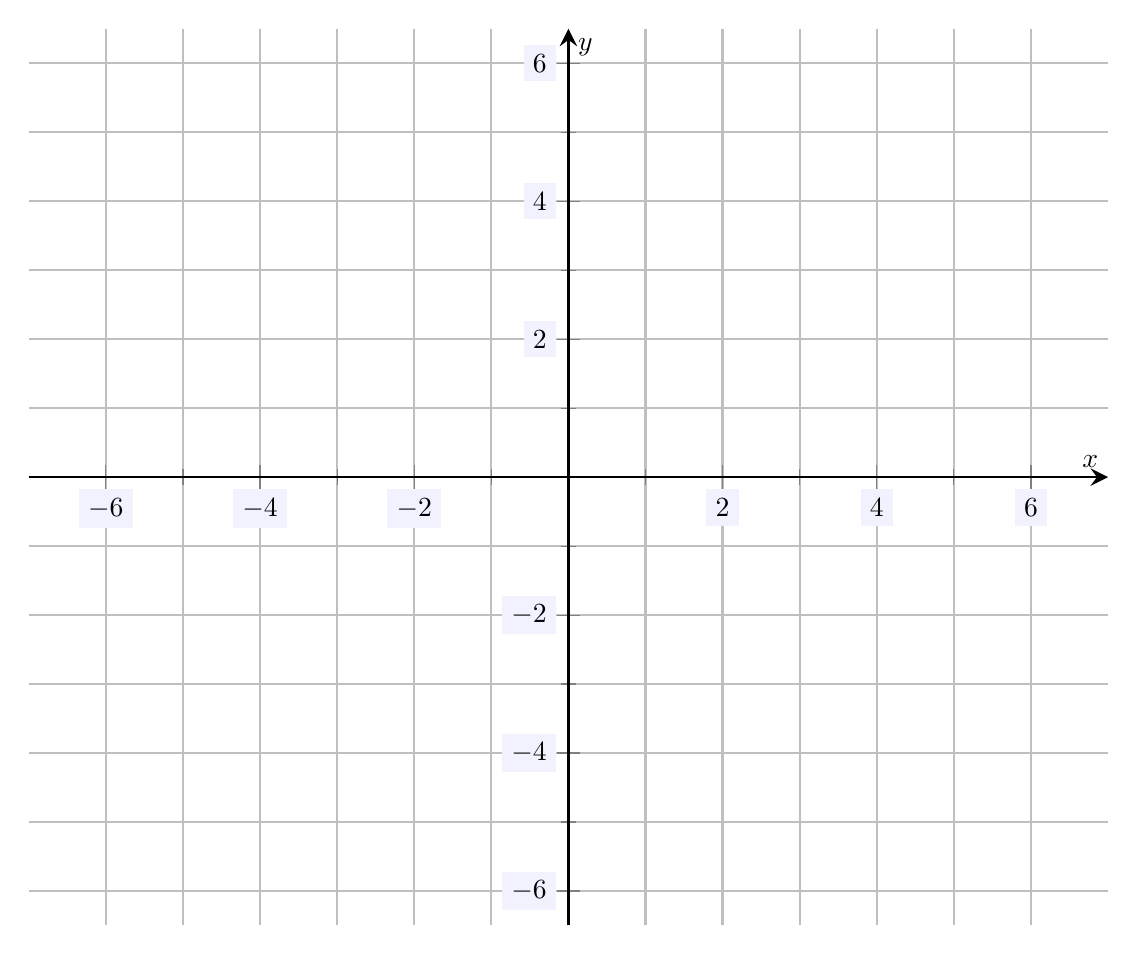
\begin{tikzpicture}[scale=2,every node/.style={scale=0.5}]
	\begin{axis}[
	grid=both,
	axis lines=middle,
	ticklabel style={fill=blue!5!white},
	xmin= -7, xmax=7,
	ymin= -6.5, ymax=6.5,
	xtick={-6,-4,-2,0,2,4,6},
	ytick={-6,-4,-2,0,2,4,6},
	minor tick = {-5,-3,...,5},
	xlabel=\(x\),ylabel=\(y\),
	]
	\end{axis}
	\end{tikzpicture}
	}
	\]





% Question 2
\newpage
\question[10] Let $f(x)$ be the quadratic function $f(x)= x^2 + 4x + 9$.
\begin{enumerate}[(a)]
\item Find the vertex and axis of symmetry for $f(x)$.
\item Does this parabola open upwards or downwards? Explain.
\item Is the function convex or concave? 
\item Does the function have a maximum or minimum value? Explain. 
\item Find the maximum or minimum value from (d). 
\end{enumerate}





% Question 3
\newpage
\question[5] Find the vertex form of $y= 3x^2 - 6x + 10$. 





% Question 4
\newpage
\question[5] Factor the polynomial $x^2 - 8x - 33$.





% Question 5
\newpage
\question[5] Factor the polynomial $2x^2 + 11x + 15$.





% Question 6
\newpage
\question[5] Consider the function $f(x)= x^2 + 6x - 40$. Find the $x$ and $y$ intercepts for this function. 





% Question 7
\newpage
\question[5] Find the solutions to $x^2= 8x - 16$.





% Question 8
\newpage
\question[5] Using the quadratic equation, find the solutions to $3 - 2x^2= 6x$. 





% Question 9
\newpage
\question[10] Consider the rational function $f(x)= \dfrac{x^2 - 25}{x^2 - x - 20}$. 
\begin{enumerate}[(a)]
\item Find the domain for $f(x)$. 
\item Find the vertical asymptotes for $f(x)$. 
\item Find the zeros for $f(x)$. 
\end{enumerate}





% Question 10
\newpage
\question[5] Compute the following, being sure to simplify as much as possible: 
	\[
	\dfrac{x + 2}{x^2 - 1} - \dfrac{4}{x^2 + 4x + 3}
	\]  





% Question 11
\newpage
\question[5] Compute the following, begin sure to simplify as much as possible:
	\[
	\dfrac{\phantom{--}\dfrac{x^2 - 4x}{x^2 - 9}\phantom{--}}{\dfrac{x^2 + 2x - 24}{x^2 + 10x + 21}}
	\] 





% Question 12
\newpage
\question[5] Solve the equation $4^{1 - x} - 3= 13$.  





% Question 13
\newpage
\question[5] Solve the equation $2e^{-x} + 5= 17$. 





% Question 14
\newpage
\question[5] Solve the equation $\log_2(x + 5)= 3$. 





% Question 15
\newpage
\question[5] Solve the equation $\log_5(x + 7) + \log_5(x + 3)= 1$. 





% Question 16
\newpage
\question[5] Suppose you invest \$500 in an account which gains 8\% annual interest, compounded semiannually. Find an expression which computes the amount of money in the account after 5~years. 





% Question 17
\newpage
\question[5] Solve the following system of equations:
	\[
	\begin{aligned}
	x - y&= 5 \\
	x + y&= 3
	\end{aligned}
	\]





% Question 18
\newpage
\question[5] Solve the following system of equations:
	\[
	\begin{aligned}
	-3x + 15y&= 9 \\
	2x + 5y&= -3
	\end{aligned}
	\]


\end{questions}
\end{document}